\begin{figure}[ht]\centering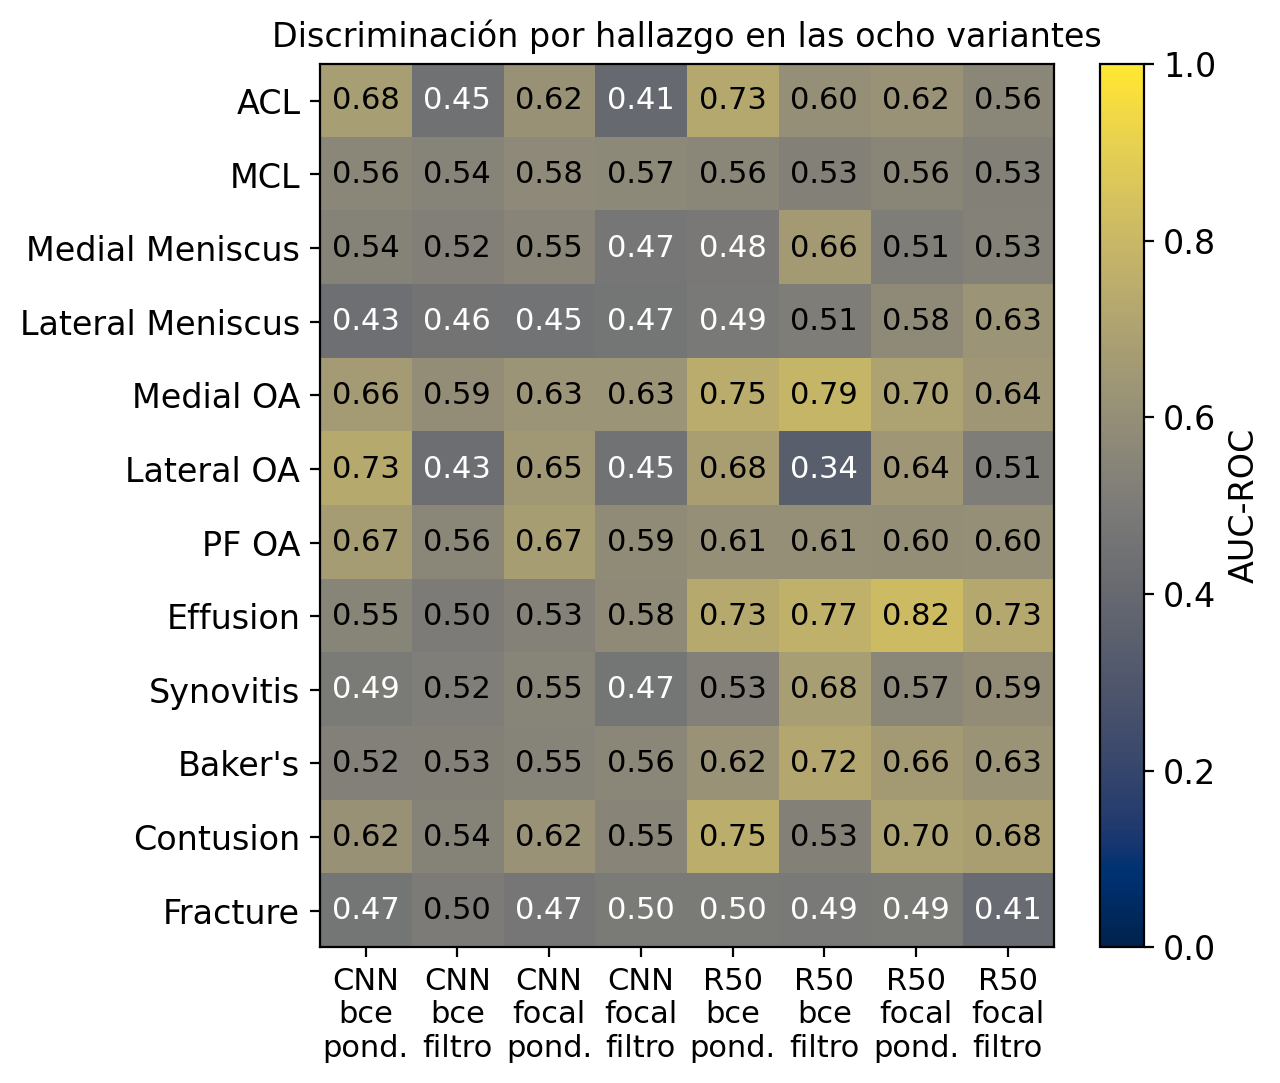
\includegraphics[width=\linewidth]{figures/auc_matrix.png}\caption{AUC por hallazgo y variante: CNN propia y R50 (ResNet-50). Las cifras y ND también están disponibles en metrics\_all\_labels.csv.}\end{figure}
\begin{figure}[ht]\centering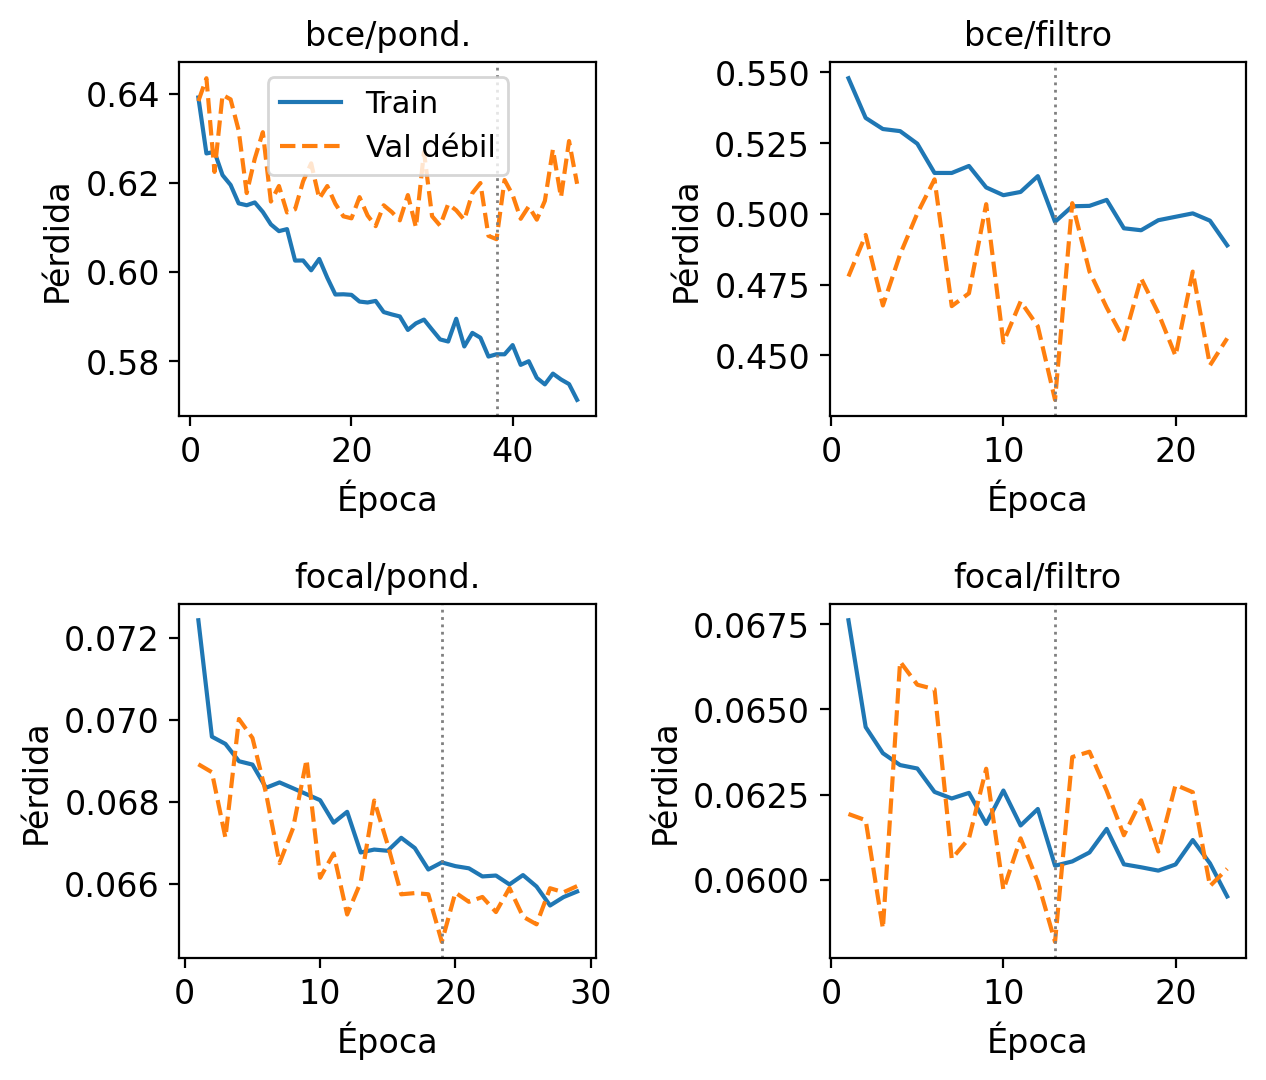
\includegraphics[width=\linewidth]{figures/curves_scratch.png}\caption{Curvas completas de la CNN propia. La línea vertical marca el checkpoint elegido. Las escalas dependen de la pérdida y no deben compararse como una misma magnitud.}\end{figure}
\begin{figure}[ht]\centering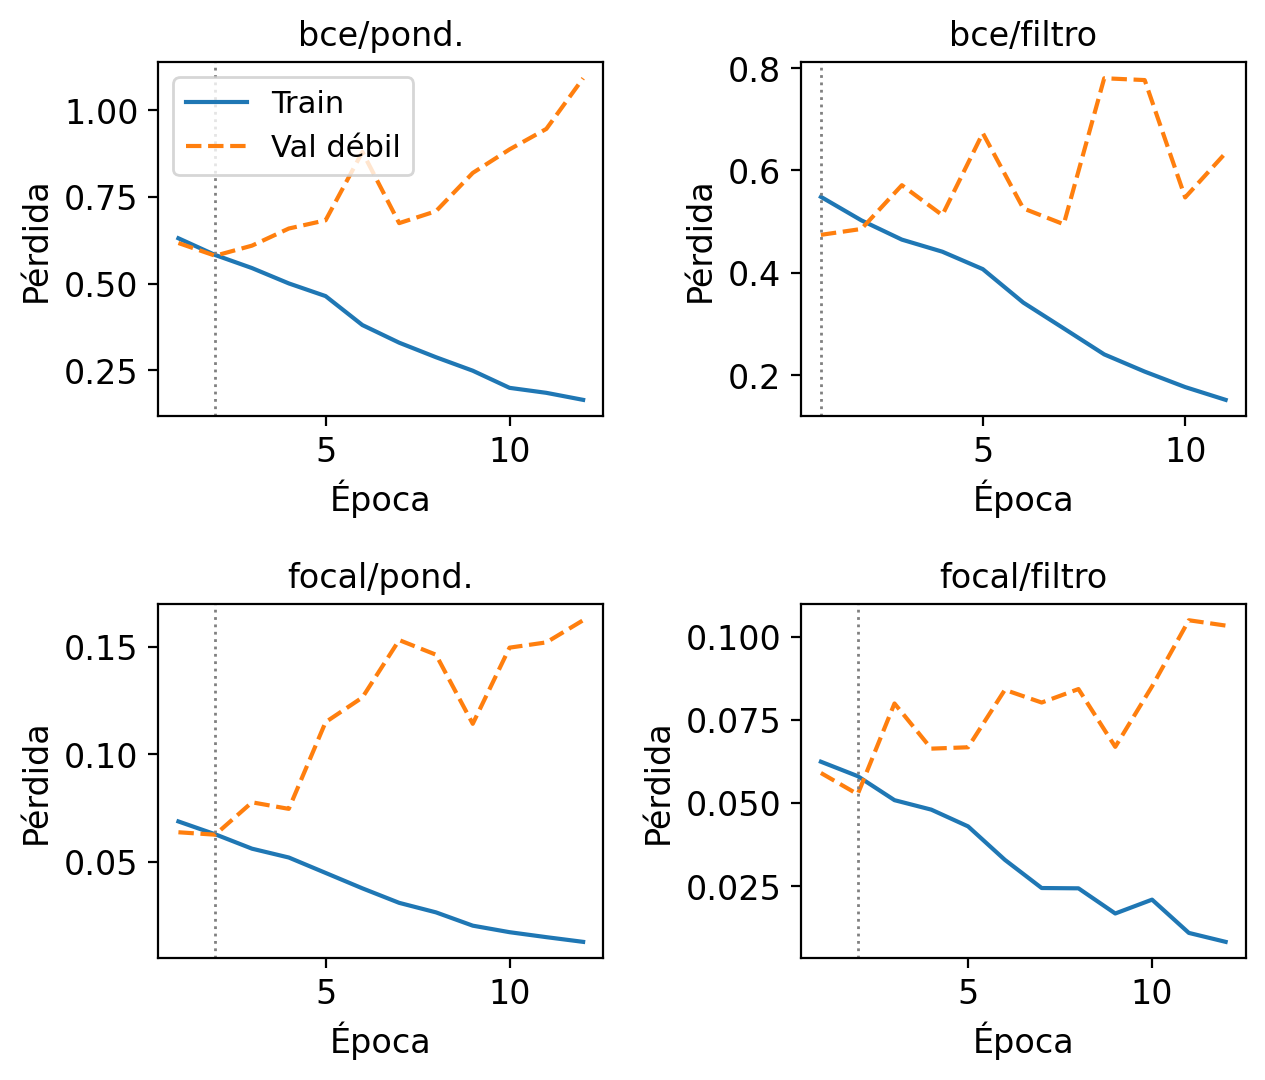
\includegraphics[width=\linewidth]{figures/curves_resnet50.png}\caption{Curvas completas de ResNet-50. La selección utiliza únicamente pérdida de validación débil, con paciencia de diez épocas.}\end{figure}
\begin{figure}[ht]\centering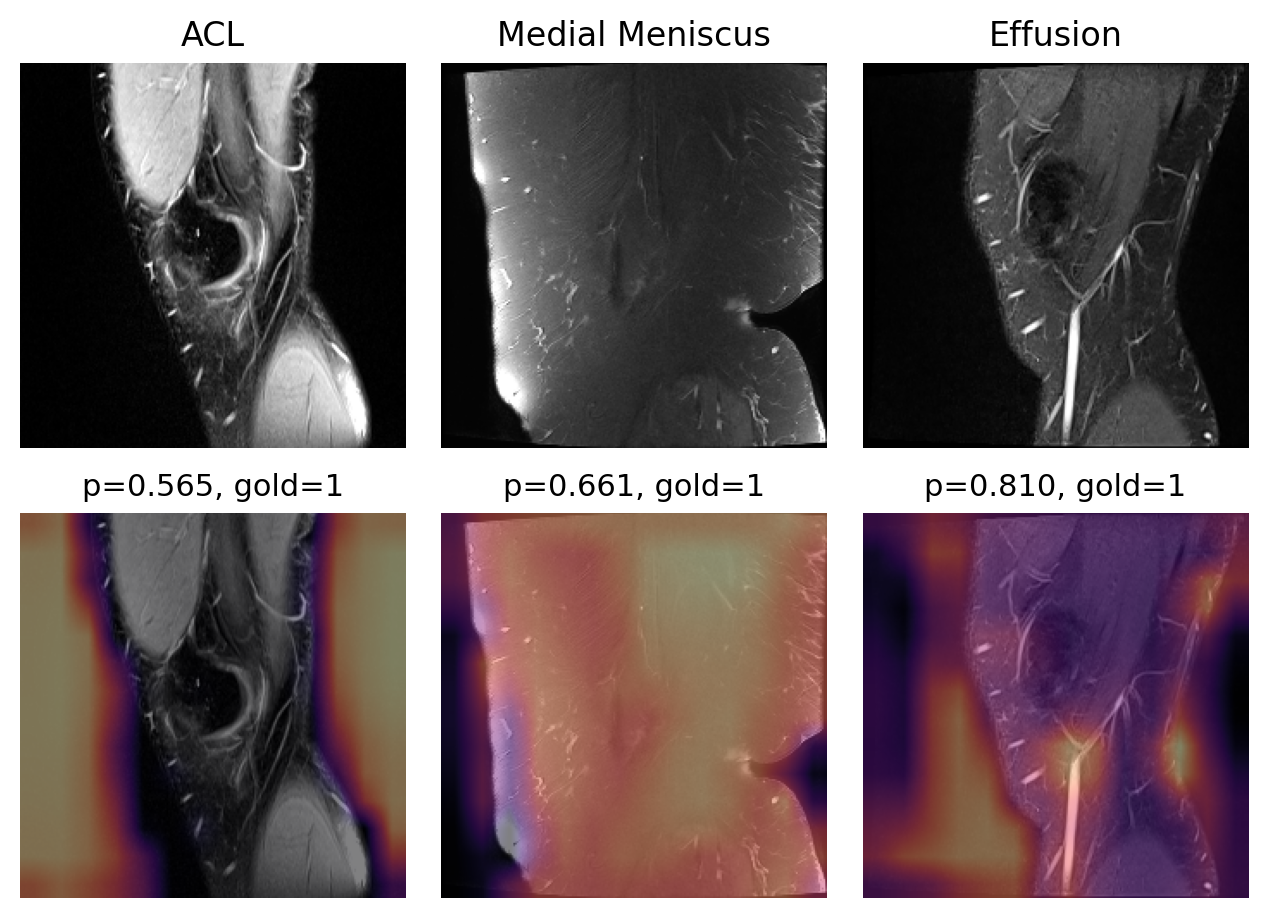
\includegraphics[width=\linewidth]{figures/cam_grid.png}\caption{Grad-CAM del baseline para tres positivos expertos, con probabilidades al umbral fijo. Casos fijados por orden del manifiesto; no elegidos por apariencia ni por acierto.}\end{figure}